\documentclass[a4paper,fontset=none]{ctexart}
\usepackage{fontspec}
\usepackage{color}
\usepackage{graphicx}
\setmainfont{Times New Roman}
\setsansfont{Noto Sans CJK SC}
\setmonofont{JetBrains Mono NL}
\setCJKmainfont{宋体}[BoldFont=Noto Sans CJK SC Bold]
\setCJKmonofont{Noto Sans Mono CJK SC}[RawFeature=+fwid]
\usepackage{indentfirst}
\setlength{\parindent}{0em}

\usepackage{listings}
\lstset{
language=Python,
basicstyle=\ttfamily\small,
aboveskip={1.0\baselineskip},
belowskip={1.0\baselineskip},
columns=fixed,
extendedchars=true,
breaklines=true,
tabsize=4,
prebreak=\raisebox{0ex}[0ex][0ex]{\ensuremath{\hookleftarrow}},
frame=lines,
showtabs=false,
showspaces=false,
showstringspaces=false,
keywordstyle=\color[rgb]{0,0.5,0},
commentstyle=\color[rgb]{0.5,0,0},
stringstyle=\color[rgb]{1,0,0},
numbers=left,
numberstyle=\small\ttfamily ,
stepnumber=1,
numbersep=12pt,
captionpos=t,
escapeinside={\%*}{*)}
}

\begin{document}

\title{\textbf{模板标题}}

\author{作者}

\date{\today}

\maketitle

\section*{Problem 1}

代码：

\lstinputlisting{Template_Code.py}

\section*{Problem 2}

代码：

\begin{lstlisting}
import numpy as np
import matplotlib.pyplot as plt
from matplotlib import cm
import math
from matplotlib.pylab import mpl
from mpl_toolkits.mplot3d import Axes3D

u = np.linspace(-3 , 3 , 101)
x , y = np.meshgrid(u , u)
print("x = \n" , x)
print("y = \n" , y)
z = np.exp(-(x**2 + y**2) / 2) / math.sqrt(2 * math.pi)

fig = plt.figure()
ax = fig.add_subplot(111, projection = '3d')
ax.plot_surface(x , y , z, rstride = 2, cstride = 2 , cmap = cm.get_cmap('winter'), linewidth = 0.5)
plt.show()
\end{lstlisting}

输出图片如下：

\begin{figure}[ht]
\centering
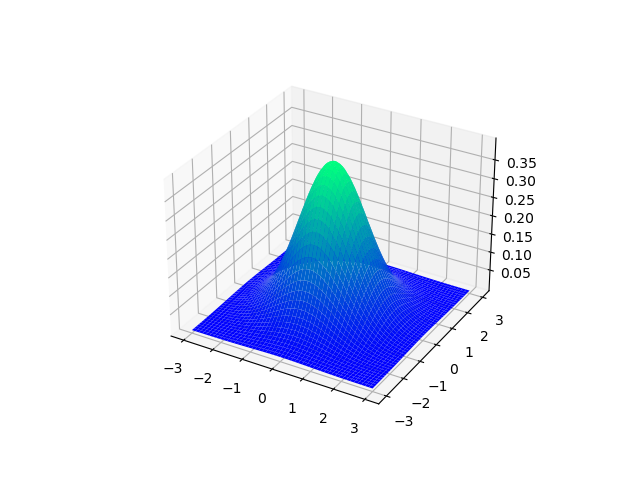
\includegraphics[width=0.8\linewidth]{Template_Picture.png}
\end{figure}

\end{document}

